\documentclass[12pt]{article}
\usepackage[utf8]{inputenc}
\usepackage[T1]{fontenc}
\usepackage{indentfirst}
\usepackage{amsmath}
\usepackage{amssymb}
\usepackage{natbib}
\usepackage{graphicx}
\usepackage{float}
\usepackage[a4paper, margin = 2 cm]{geometry}
\usepackage{fancyhdr}
\usepackage{wrapfig}
\usepackage{hyperref}

\title{JAiO zadanie 4}
\author{Dominik Wawszczak}
\date{2023-06-06}

\begin{document}
	\setlength{\parindent}{0 cm}
	
	Kacper Bal 439948 \hfill Zadanie 1
	
	Piotr Blinowski 439949
	
	Dominik Wawszczak 440014
	
	\bigskip
	\hrule
	\bigskip
	
	Udowodnimy, że język
	\[ L \ = \ \left( \left\{ a^{n} b^{n} \ : \ n \in \mathbb{Z}^{+} \cup
	\left\{ 0 \right\} \right\} \right) ^ {\ast} \]
	nie jest rozpoznowany przez żaden automat ze stosem pracujący w skończenie
	wielu fazach.
	
	\medskip
	
	Na początek udowodnimy, że \(L \in \text{CFL}\). Weźmy gramatykę
	\(\mathcal{G} = \left( \left\{ a, b \right\}, \left\{ S, T \right\}, P, S
	\right)\) z produkcjami:
	\begin{itemize}
		\item \(S \longrightarrow SS \mid T \mid \varepsilon\),
		\item \(T \longrightarrow aTb \mid \varepsilon\).
	\end{itemize}
	Łatwo widać, że gramatyka \(\mathcal{G}\) opisuje język \(L\), jednak nie
	będziemy zagłębiać się w szczegóły. Wynika z tego, że \(L \in \text{CFL}\).
	
	\medskip
	
	Przypuśćmy nie wprost, że istnieje automat ze stosem \(\mathcal{A}\) o
	zbiorze stanów \(Q\) i zbiorze symboli stosowych \(\Gamma\), działający w co
	najwyżej \(k\) fazach, rozpoznający język \(L\). Przez resztę rozwiązania
	zadania będziemy działać na słowie \(w = \left( a^{X} b^{X} \right) ^ {Y}
	\in L\), gdzie \(X = \left( 21 \cdot \left| Q \right| \cdot \left| \Gamma
	\right| + 37 \right) ^ {2}\), a \(Y = 69 \cdot k \cdot X + 420\).
	
	\medskip
	
	Wprowadźmy następujące definicje:
	\begin{itemize}
		\item \textit{długością} fazy nazwiemy liczbę przejść, które dana faza
		      zawiera, przy czym uwzględniamy tutaj zarówno przejścia po
		      literach czytanego słowa, jak i \(\varepsilon\)-przejścia;
		\item \textit{zmianą} fazy nazwiemy wartość bezwzględną różnicy rozmiaru
		      stosu na początku i na końcu fazy.
	\end{itemize}
	
	\medskip
	
	\textbf{Lemat 1}
	
	W biegu akceptującym automatu \(\mathcal{A}\) po słowie \(w\), w ramach
	jednej fazy nie może być ciągu \(\left| Q \right|\) kolejnych przejść
	niezmieniających stosu. Zakładamy przy tym, że wspomniany bieg nie ma
	\(\varepsilon\)-przejść niezmieniających stanu ani stosu, ponieważ gdyby
	miał, to możnaby je usunąć.
	
	\medskip
	
	\textbf{Dowód Lematu 1}
	
	Przypuśćmy nie wprost, że w pewnej fazie wystąpiło \(\left| Q \right|\)
	kolejnych przejść niezmieniających stosu. Wówczas z Zasady Szufladkowej
	Dirichleta wynika, że wśród tych przejść pewien stan \(q\) wystąpił co
	najmniej dwa razy, gdyż łącznie automat przeszedł przez \(\left| Q
	\right| + 1\) stanów. Zauważmy, że słowo wczytane w tym okresie jest
	niepuste, ponieważ założyliśmy, że nie ma \(\varepsilon\) przejść
	niezmieniających stanu ani stosu. Łatwo widać, że słowo to można napompować,
	a skoro ma ono długość co najwyżej \(\left| Q \right|\), to z pewnością nie
	jest ono postaci \(\left( a^{X} b^{X} \right) ^ m\), dla pewnego \(m \in
	\mathbb{Z}^{+}\), zatem na skutek tego pompowania powstanie nowe słowo
	nienależące do \(L\), po którym będzie istniał bieg akceptujący automatu
	\(\mathcal{A}\). Otrzymana sprzeczność końćzy dowód lematu.
	
	\medskip
	
	\textbf{Lemat 2}
	
	\[ \text{Jeśli faza ma długość} \ n
	\text{, to jej zmiana należy do przedziału} \ \left[ \left\lfloor
	\frac{n}{\left| Q \right|} \right\rfloor, n \right] \text{.} \]
	Lemat ten jest bezpośrednim wnioskiem z lematu 1.
	
	\medskip
	
	Zauważmy, że w biegu akceptującym automatu \(\mathcal{A}\) po słowie \(w\)
	musi istnieć faza push długości co najmniej \(3X\), co wynika z doboru
	stałej \(Y\), ponieważ w przeciwnym wypadku z lematu 2 musiałby być wykonany
	pop na pustym stosie. W trakcie tej fazy wczytany więc zostanie pełny blok
	\(b^{X}\). Z doboru stałej \(X\) oraz Zasady Szufladkowej Dirichleta wynika,
	że w trakcie przechodzenia tej fazy przez blok \(b^{X}\) \(\left| Q \right|
	+ 1\) razy wystąpi moment, że aktualny stan to pewne \(q\), a aktualny
	symbol na szczycie stosu to pewne \(s\). Ponownie, wczytane słowo pomiędzy
	każdymi dwoma momentami jest niepuste, a dodatkowo ma długość co najwyżej
	\(\left| Q \right| \cdot \left| \Gamma \right|\) i składa się z samych liter
	\(b\). Stos natomiast pomiędzy momentami \(i\)-tym a \(i + 1\)-szym
	powiększy się o pewne słowo \(v_{i}\) długości również co najwyżej \(\left|
	Q \right| \cdot \left| \Gamma \right|\), którego ostatnia litera to
	oczywiście \(s\).
	\begin{center}
		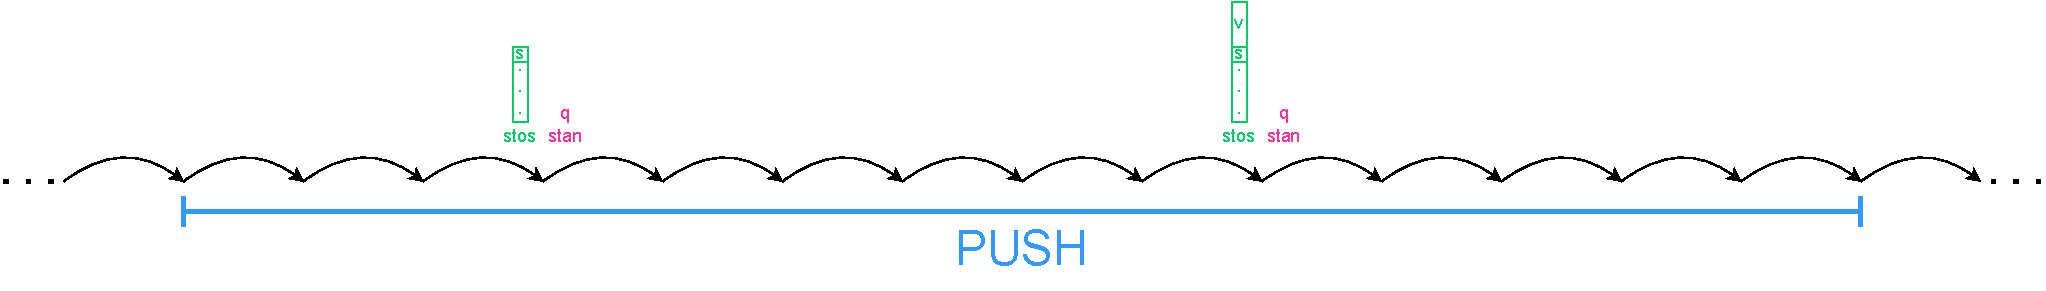
\includegraphics[width = 0.9 \textwidth]{./image-1.pdf}
	\end{center}
	
	\medskip
	
	Rozważmy dwa przypadki:
	\begin{enumerate}
		\item Symbol \(s\) do końca biegu automatu pozostaje na stosie.
		      
		      Łatwo wówczas zauważyć, że możemy podwoić słowo złożone
		      przeczytane pomiędzy pierwszym a drugim momentem, uzyskując w ten
		      sposób nowe słowo \(w' \notin L\), bo podwojony fragment składa
		      się z samych liter \(b\). Słowo to zostanie zwyczajnie
		      zaakceptowane przez automat \(\mathcal{A}\), gdyż podwojony
		      fragment dopisuje tylko słowo \(v_{1}\) do stosu, a skoro litera
		      bezpośrednio pod tym słowem nie zostanie zdjęta, to z perspektywy
		      automatu nie będzie różnicy, czyli sprzeczność, ponieważ automat
		      \(\mathcal{A}\) zaakceptuje słowo nienależące do \(L\).
		
		\item W przeciwnym wypadku, każde ze słów \(v_{1}, v_{2}, \ldots,
		      v_{\left| Q \right|}\) zostanie kiedyś ze stosu zdjęte. Innymi
		      słowy, istnieje spójny fragment ciągu przejść odpowiadający za
		      zdjecie ze stosu słowa \(v_{1} v_{2} \ldots v_{\left| Q
		      \right|}\). Bardziej formalnie, na początku tego ciągu stos jest
		      postaci \(pref \cdot v_{1} v_{2} \ldots v_{\left| Q \right|}\), a
		      na koniec po prostu \(pref\). W trakcie natomiast na stosie mogą
		      być wykonywane zarówno operacje push, jak i pop. Fragment ten
		      można podzielić na \(\left| Q \right|\) mniejszych fragmentów w
		      taki sposób, że w \(i\)-tym ze stosu zostaje zdjęte słowo
		      \(v_{i}\) (,,zdjęte'' jako efekt końcowy -- w trakcie mogą dziać
		      się różne rzeczy).
		      
		      \medskip
		      
		      Każdy z tych fragmentów kończy w jakimś stanie, z którego
		      następnie rozpoczyna się kolejny fragment. Z Zasady Szufladkowej
		      Dirichleta wynika, że pewne dwa z tych stanów będą takie same.
		      Możemy podwoić konkatenację liter odpowiadających fragmentom
		      pomiędzy nimi, jednocześnie podwajając litery przeczytane przez
		      stos z odpowiedniego fragmentu wspomnianej wcześniej fazy push.
		      Oczywiście, jak zostało zaznaczone wcześniej, będą to tylko litery
		      \(b\). W tym przypadku zatem również otrzymamy nowe słowo \(w'
		      \notin L\), które automat zaakceptuje, gdyż z jego perspektywy
		      nie będzie różnicy -- wykonuje przejścia w oparciu jedynie o
		      aktualny stan, symbol na szczycie stosu i czytaną literę. W tym
		      przypadku jednak nieco trudniejsze jest zauważenie, że \(w' \notin
		      L\). Wynika to z tego, że podwojona lewa część składa się z samych
		      liter \(b\), zatem liczba tych liter w nowym bloku \(b\) z
		      pewnością będzie różna od liczby liter \(a\) w bloku poprzednim.
	\end{enumerate}
	
	\medskip
	
	Z powyższego wynika, że automaty ze stosem pracujące w skończenie wielu
	fazach nie rozpoznają wszystkich języków bezkontekstowych (w szczególności
	\(L\)), co kończy rozwiązanie zadania.
	\begin{flushright}
		\(\Box\)
	\end{flushright}
\end{document}
